\documentclass[twoside]{book}

% Packages required by doxygen
\usepackage{fixltx2e}
\usepackage{calc}
\usepackage{doxygen}
\usepackage[export]{adjustbox} % also loads graphicx
\usepackage{graphicx}
\usepackage[utf8]{inputenc}
\usepackage{makeidx}
\usepackage{multicol}
\usepackage{multirow}
\PassOptionsToPackage{warn}{textcomp}
\usepackage{textcomp}
\usepackage[nointegrals]{wasysym}
\usepackage[table]{xcolor}

% Font selection
\usepackage[T1]{fontenc}
\usepackage[scaled=.90]{helvet}
\usepackage{courier}
\usepackage{amssymb}
\usepackage{sectsty}
\renewcommand{\familydefault}{\sfdefault}
\allsectionsfont{%
  \fontseries{bc}\selectfont%
  \color{darkgray}%
}
\renewcommand{\DoxyLabelFont}{%
  \fontseries{bc}\selectfont%
  \color{darkgray}%
}
\newcommand{\+}{\discretionary{\mbox{\scriptsize$\hookleftarrow$}}{}{}}

% Page & text layout
\usepackage{geometry}
\geometry{%
  a4paper,%
  top=2.5cm,%
  bottom=2.5cm,%
  left=2.5cm,%
  right=2.5cm%
}
\tolerance=750
\hfuzz=15pt
\hbadness=750
\setlength{\emergencystretch}{15pt}
\setlength{\parindent}{0cm}
\setlength{\parskip}{3ex plus 2ex minus 2ex}
\makeatletter
\renewcommand{\paragraph}{%
  \@startsection{paragraph}{4}{0ex}{-1.0ex}{1.0ex}{%
    \normalfont\normalsize\bfseries\SS@parafont%
  }%
}
\renewcommand{\subparagraph}{%
  \@startsection{subparagraph}{5}{0ex}{-1.0ex}{1.0ex}{%
    \normalfont\normalsize\bfseries\SS@subparafont%
  }%
}
\makeatother

% Headers & footers
\usepackage{fancyhdr}
\pagestyle{fancyplain}
\fancyhead[LE]{\fancyplain{}{\bfseries\thepage}}
\fancyhead[CE]{\fancyplain{}{}}
\fancyhead[RE]{\fancyplain{}{\bfseries\leftmark}}
\fancyhead[LO]{\fancyplain{}{\bfseries\rightmark}}
\fancyhead[CO]{\fancyplain{}{}}
\fancyhead[RO]{\fancyplain{}{\bfseries\thepage}}
\fancyfoot[LE]{\fancyplain{}{}}
\fancyfoot[CE]{\fancyplain{}{}}
\fancyfoot[RE]{\fancyplain{}{\bfseries\scriptsize Generated by Doxygen }}
\fancyfoot[LO]{\fancyplain{}{\bfseries\scriptsize Generated by Doxygen }}
\fancyfoot[CO]{\fancyplain{}{}}
\fancyfoot[RO]{\fancyplain{}{}}
\renewcommand{\footrulewidth}{0.4pt}
\renewcommand{\chaptermark}[1]{%
  \markboth{#1}{}%
}
\renewcommand{\sectionmark}[1]{%
  \markright{\thesection\ #1}%
}

% Indices & bibliography
\usepackage{natbib}
\usepackage[titles]{tocloft}
\setcounter{tocdepth}{3}
\setcounter{secnumdepth}{5}
\makeindex

% Hyperlinks (required, but should be loaded last)
\usepackage{ifpdf}
\ifpdf
  \usepackage[pdftex,pagebackref=true]{hyperref}
\else
  \usepackage[ps2pdf,pagebackref=true]{hyperref}
\fi
\hypersetup{%
  colorlinks=true,%
  linkcolor=blue,%
  citecolor=blue,%
  unicode%
}

% Custom commands
\newcommand{\clearemptydoublepage}{%
  \newpage{\pagestyle{empty}\cleardoublepage}%
}

\usepackage{caption}
\captionsetup{labelsep=space,justification=centering,font={bf},singlelinecheck=off,skip=4pt,position=top}

%===== C O N T E N T S =====

\begin{document}

% Titlepage & ToC
\hypersetup{pageanchor=false,
             bookmarksnumbered=true,
             pdfencoding=unicode
            }
\pagenumbering{alph}
\begin{titlepage}
\vspace*{7cm}
\begin{center}%
{\Large My Project }\\
\vspace*{1cm}
{\large Generated by Doxygen 1.8.13}\\
\end{center}
\end{titlepage}
\clearemptydoublepage
\pagenumbering{roman}
\tableofcontents
\clearemptydoublepage
\pagenumbering{arabic}
\hypersetup{pageanchor=true}

%--- Begin generated contents ---
\chapter{Hierarchical Index}
\section{Class Hierarchy}
This inheritance list is sorted roughly, but not completely, alphabetically\+:\begin{DoxyCompactList}
\item \contentsline{section}{Point}{\pageref{classPoint}}{}
\item \contentsline{section}{Poligono}{\pageref{classPoligono}}{}
\begin{DoxyCompactList}
\item \contentsline{section}{Retangulo}{\pageref{classRetangulo}}{}
\end{DoxyCompactList}
\end{DoxyCompactList}

\chapter{Class Index}
\section{Class List}
Here are the classes, structs, unions and interfaces with brief descriptions\+:\begin{DoxyCompactList}
\item\contentsline{section}{\hyperlink{classPoint}{Point} }{\pageref{classPoint}}{}
\item\contentsline{section}{\hyperlink{classPoligono}{Poligono} }{\pageref{classPoligono}}{}
\item\contentsline{section}{\hyperlink{classRetangulo}{Retangulo} }{\pageref{classRetangulo}}{}
\end{DoxyCompactList}

\chapter{Class Documentation}
\hypertarget{classPoint}{}\section{Point Class Reference}
\label{classPoint}\index{Point@{Point}}
\subsection*{Public Member Functions}
\begin{DoxyCompactItemize}
\item 
\mbox{\Hypertarget{classPoint_a30773ae254834ba9ce4661bf492cd07a}\label{classPoint_a30773ae254834ba9ce4661bf492cd07a}} 
{\bfseries Point} (float mx=0, float my=0)
\item 
\mbox{\Hypertarget{classPoint_af0c0f20db1616447bc78184ed537ef6e}\label{classPoint_af0c0f20db1616447bc78184ed537ef6e}} 
{\bfseries Point} (const \hyperlink{classPoint}{Point} \&p)
\item 
\mbox{\Hypertarget{classPoint_acee4acaa1d515e9973145f977e500fe6}\label{classPoint_acee4acaa1d515e9973145f977e500fe6}} 
void {\bfseries setX} (float mx)
\item 
\mbox{\Hypertarget{classPoint_a756b3f64d961a5059302f42e1fcf2332}\label{classPoint_a756b3f64d961a5059302f42e1fcf2332}} 
void {\bfseries setY} (float my)
\item 
\mbox{\Hypertarget{classPoint_afe2b937778d9fe5c135ab61de91271e9}\label{classPoint_afe2b937778d9fe5c135ab61de91271e9}} 
void {\bfseries set\+XY} (float mx, float my)
\item 
\mbox{\Hypertarget{classPoint_a29c44ec7c7279e02629645a06cdaf7d5}\label{classPoint_a29c44ec7c7279e02629645a06cdaf7d5}} 
float {\bfseries getX} () const
\item 
\mbox{\Hypertarget{classPoint_a2371ffadbe245d12a8f556d0a976521b}\label{classPoint_a2371ffadbe245d12a8f556d0a976521b}} 
float {\bfseries getY} () const
\item 
\mbox{\Hypertarget{classPoint_a039e6b445145494242cf2baa3895bcf7}\label{classPoint_a039e6b445145494242cf2baa3895bcf7}} 
\hyperlink{classPoint}{Point} {\bfseries add} (\hyperlink{classPoint}{Point} P1)
\item 
\mbox{\Hypertarget{classPoint_a01d301ef29a031f0ce7df37c2da12e49}\label{classPoint_a01d301ef29a031f0ce7df37c2da12e49}} 
\hyperlink{classPoint}{Point} {\bfseries sub} (\hyperlink{classPoint}{Point} P1)
\item 
\mbox{\Hypertarget{classPoint_abd2618d1f505d9392893273a66e7c9b2}\label{classPoint_abd2618d1f505d9392893273a66e7c9b2}} 
float {\bfseries norma} ()
\item 
\mbox{\Hypertarget{classPoint_a8fc932c5dcb7ef85208b01f7efa83163}\label{classPoint_a8fc932c5dcb7ef85208b01f7efa83163}} 
\hyperlink{classPoint}{Point} {\bfseries translada} (float a, float b)
\item 
\mbox{\Hypertarget{classPoint_a1fb5c2501c27ab2cbc99d06c2a26a741}\label{classPoint_a1fb5c2501c27ab2cbc99d06c2a26a741}} 
void {\bfseries imprime} ()
\end{DoxyCompactItemize}
\subsection*{Friends}
\begin{DoxyCompactItemize}
\item 
\mbox{\Hypertarget{classPoint_af113210dbdf59ad1a6621e2e30e14aea}\label{classPoint_af113210dbdf59ad1a6621e2e30e14aea}} 
ostream \& {\bfseries operator$<$$<$} (ostream \&X, const \hyperlink{classPoint}{Point} \&H)
\end{DoxyCompactItemize}


The documentation for this class was generated from the following files\+:\begin{DoxyCompactItemize}
\item 
point\+\_\+class.\+h\item 
point\+\_\+class.\+cpp\end{DoxyCompactItemize}

\hypertarget{classPoligono}{}\section{Poligono Class Reference}
\label{classPoligono}\index{Poligono@{Poligono}}


Inheritance diagram for Poligono\+:\nopagebreak
\begin{figure}[H]
\begin{center}
\leavevmode
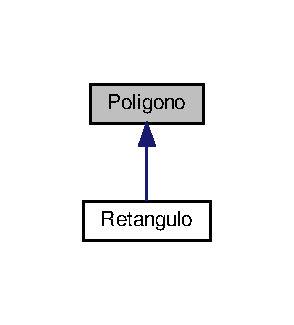
\includegraphics[width=141pt]{classPoligono__inherit__graph}
\end{center}
\end{figure}
\subsection*{Public Member Functions}
\begin{DoxyCompactItemize}
\item 
\hyperlink{classPoligono_a9311a9a1496878c09c8508b3636e2870}{Poligono} ()
\begin{DoxyCompactList}\small\item\em contrutores inline \end{DoxyCompactList}\item 
\hyperlink{classPoligono_a7d2e73767b8dc1bce595f0f286d0e85a}{Poligono} (const \hyperlink{classPoligono}{Poligono} \&Pol)
\item 
\hyperlink{classPoligono_a4dd7136ee506cb4355cbdc724c55a4a0}{$\sim$\+Poligono} ()
\item 
void \hyperlink{classPoligono_a15dd684ea903a4eb5ba8671d57facb82}{setV} (float x, float y)
\begin{DoxyCompactList}\small\item\em metodos \end{DoxyCompactList}\item 
unsigned \hyperlink{classPoligono_abb6eef3e304cb28501356fd5512b0890}{getN} ()
\item 
void \hyperlink{classPoligono_adbf605dfd0419b7301c9be0ec1dbe41b}{translada} (float a, float b)
\item 
double \hyperlink{classPoligono_a76e434d95055f6c94fdcf3c314d44be0}{Area} ()
\item 
void \hyperlink{classPoligono_a8c696d750b78769e9b2e04790dac9195}{printpol} ()
\item 
void \hyperlink{classPoligono_a8891a75b7f11bd764a99f296145e26dd}{rotation} (\hyperlink{classPoint}{Point} P1, float ang)
\item 
\hyperlink{classPoint}{Point} \hyperlink{classPoligono_a9f5148c45bc074be28664efc717e5968}{cmass} ()
\end{DoxyCompactItemize}


\subsection{Constructor \& Destructor Documentation}
\mbox{\Hypertarget{classPoligono_a9311a9a1496878c09c8508b3636e2870}\label{classPoligono_a9311a9a1496878c09c8508b3636e2870}} 
\index{Poligono@{Poligono}!Poligono@{Poligono}}
\index{Poligono@{Poligono}!Poligono@{Poligono}}
\subsubsection{\texorpdfstring{Poligono()}{Poligono()}\hspace{0.1cm}{\footnotesize\ttfamily [1/2]}}
{\footnotesize\ttfamily Poligono\+::\+Poligono (\begin{DoxyParamCaption}{ }\end{DoxyParamCaption})\hspace{0.3cm}{\ttfamily [inline]}}



contrutores inline 

construtor por default\+: inicia o poligono sem nenhum ponto cadastrado \mbox{\Hypertarget{classPoligono_a7d2e73767b8dc1bce595f0f286d0e85a}\label{classPoligono_a7d2e73767b8dc1bce595f0f286d0e85a}} 
\index{Poligono@{Poligono}!Poligono@{Poligono}}
\index{Poligono@{Poligono}!Poligono@{Poligono}}
\subsubsection{\texorpdfstring{Poligono()}{Poligono()}\hspace{0.1cm}{\footnotesize\ttfamily [2/2]}}
{\footnotesize\ttfamily Poligono\+::\+Poligono (\begin{DoxyParamCaption}\item[{const \hyperlink{classPoligono}{Poligono} \&}]{Pol }\end{DoxyParamCaption})\hspace{0.3cm}{\ttfamily [inline]}}

construtor por parâmetro\+: inicia o poligono com os pontos que estam no poligono que foi passado como parâmetro \mbox{\Hypertarget{classPoligono_a4dd7136ee506cb4355cbdc724c55a4a0}\label{classPoligono_a4dd7136ee506cb4355cbdc724c55a4a0}} 
\index{Poligono@{Poligono}!````~Poligono@{$\sim$\+Poligono}}
\index{````~Poligono@{$\sim$\+Poligono}!Poligono@{Poligono}}
\subsubsection{\texorpdfstring{$\sim$\+Poligono()}{~Poligono()}}
{\footnotesize\ttfamily Poligono\+::$\sim$\+Poligono (\begin{DoxyParamCaption}{ }\end{DoxyParamCaption})\hspace{0.3cm}{\ttfamily [inline]}}

destrutor\+: zera todos os verticies do poligono 

\subsection{Member Function Documentation}
\mbox{\Hypertarget{classPoligono_a76e434d95055f6c94fdcf3c314d44be0}\label{classPoligono_a76e434d95055f6c94fdcf3c314d44be0}} 
\index{Poligono@{Poligono}!Area@{Area}}
\index{Area@{Area}!Poligono@{Poligono}}
\subsubsection{\texorpdfstring{Area()}{Area()}}
{\footnotesize\ttfamily double Poligono\+::\+Area (\begin{DoxyParamCaption}{ }\end{DoxyParamCaption})}

metodo responsável por calcular a Área do poligono metodo não recebe nada como parâmetro mas retorna o valor da área do tipo double \mbox{\Hypertarget{classPoligono_a9f5148c45bc074be28664efc717e5968}\label{classPoligono_a9f5148c45bc074be28664efc717e5968}} 
\index{Poligono@{Poligono}!cmass@{cmass}}
\index{cmass@{cmass}!Poligono@{Poligono}}
\subsubsection{\texorpdfstring{cmass()}{cmass()}}
{\footnotesize\ttfamily \hyperlink{classPoint}{Point} Poligono\+::cmass (\begin{DoxyParamCaption}{ }\end{DoxyParamCaption})}

metodo responsável por calcular o centro de massa do poligono não recebe nenhum argumento mas retorna o ponto do centro de massa \mbox{\Hypertarget{classPoligono_abb6eef3e304cb28501356fd5512b0890}\label{classPoligono_abb6eef3e304cb28501356fd5512b0890}} 
\index{Poligono@{Poligono}!getN@{getN}}
\index{getN@{getN}!Poligono@{Poligono}}
\subsubsection{\texorpdfstring{get\+N()}{getN()}}
{\footnotesize\ttfamily unsigned Poligono\+::getN (\begin{DoxyParamCaption}{ }\end{DoxyParamCaption})\hspace{0.3cm}{\ttfamily [inline]}}

metodo responsável por retornar o número de verticies do poligono nao recebe argumentos mas retorna o numero de verticies do tipo unsigned int \mbox{\Hypertarget{classPoligono_a8c696d750b78769e9b2e04790dac9195}\label{classPoligono_a8c696d750b78769e9b2e04790dac9195}} 
\index{Poligono@{Poligono}!printpol@{printpol}}
\index{printpol@{printpol}!Poligono@{Poligono}}
\subsubsection{\texorpdfstring{printpol()}{printpol()}}
{\footnotesize\ttfamily void Poligono\+::printpol (\begin{DoxyParamCaption}{ }\end{DoxyParamCaption})}

metodo responsável por imprimir o poligono \mbox{\Hypertarget{classPoligono_a8891a75b7f11bd764a99f296145e26dd}\label{classPoligono_a8891a75b7f11bd764a99f296145e26dd}} 
\index{Poligono@{Poligono}!rotation@{rotation}}
\index{rotation@{rotation}!Poligono@{Poligono}}
\subsubsection{\texorpdfstring{rotation()}{rotation()}}
{\footnotesize\ttfamily void Poligono\+::rotation (\begin{DoxyParamCaption}\item[{\hyperlink{classPoint}{Point}}]{P1,  }\item[{float}]{ang }\end{DoxyParamCaption})}

metodo responsável por rotacionar o poligono com base no ponto que for passado como parâmetro metodo recebe como parâmetro o ponto que será a base para a rotação e o ângulo o qual o poligono será rotacionado \mbox{\Hypertarget{classPoligono_a15dd684ea903a4eb5ba8671d57facb82}\label{classPoligono_a15dd684ea903a4eb5ba8671d57facb82}} 
\index{Poligono@{Poligono}!setV@{setV}}
\index{setV@{setV}!Poligono@{Poligono}}
\subsubsection{\texorpdfstring{set\+V()}{setV()}}
{\footnotesize\ttfamily void Poligono\+::setV (\begin{DoxyParamCaption}\item[{float}]{mx,  }\item[{float}]{my }\end{DoxyParamCaption})}



metodos 

metodo responsável por cadastrar um novo verticie ao polinômio. metodo recebe como parâmetro as cordenadas x e y do novo verticie. \mbox{\Hypertarget{classPoligono_adbf605dfd0419b7301c9be0ec1dbe41b}\label{classPoligono_adbf605dfd0419b7301c9be0ec1dbe41b}} 
\index{Poligono@{Poligono}!translada@{translada}}
\index{translada@{translada}!Poligono@{Poligono}}
\subsubsection{\texorpdfstring{translada()}{translada()}}
{\footnotesize\ttfamily void Poligono\+::translada (\begin{DoxyParamCaption}\item[{float}]{a,  }\item[{float}]{b }\end{DoxyParamCaption})}

metodo responsável por transladar o poligono para um determinada posição definida pelo usuário metodo recebe como parâmetro as distancias a e b, as mesmas serão somadas a todos os pontos do poligono da seguinte forma\+: condenada x+a e cordenada y+b. 

The documentation for this class was generated from the following files\+:\begin{DoxyCompactItemize}
\item 
poligono\+\_\+class.\+h\item 
poligono\+\_\+class.\+cpp\end{DoxyCompactItemize}

\hypertarget{classRetangulo}{}\section{Retangulo Class Reference}
\label{classRetangulo}\index{Retangulo@{Retangulo}}


Inheritance diagram for Retangulo\+:\nopagebreak
\begin{figure}[H]
\begin{center}
\leavevmode
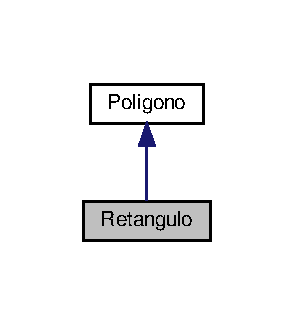
\includegraphics[width=141pt]{classRetangulo__inherit__graph}
\end{center}
\end{figure}


Collaboration diagram for Retangulo\+:\nopagebreak
\begin{figure}[H]
\begin{center}
\leavevmode
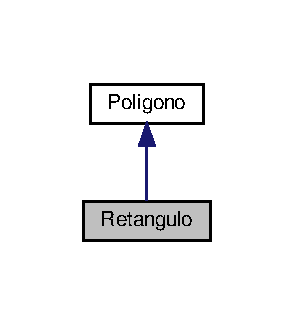
\includegraphics[width=141pt]{classRetangulo__coll__graph}
\end{center}
\end{figure}
\subsection*{Public Member Functions}
\begin{DoxyCompactItemize}
\item 
\mbox{\Hypertarget{classRetangulo_a563778613d1b13d6d3056aca22ab22cd}\label{classRetangulo_a563778613d1b13d6d3056aca22ab22cd}} 
{\bfseries Retangulo} (float mx=0, float my=0, float \+\_\+altura=0, float \+\_\+largura=0)
\end{DoxyCompactItemize}


The documentation for this class was generated from the following files\+:\begin{DoxyCompactItemize}
\item 
retangulo\+\_\+class.\+h\item 
retangulo\+\_\+class.\+cpp\end{DoxyCompactItemize}

%--- End generated contents ---

% Index
\backmatter
\newpage
\phantomsection
\clearemptydoublepage
\addcontentsline{toc}{chapter}{Index}
\printindex

\end{document}
